% !TEX TS-program = XeLaTeX
\documentclass[a4paper]{article}

% https://tex.stackexchange.com/a/5365
% Must
\usepackage[table]{xcolor}

\usepackage{tabularx}


\usepackage{tikz}
\usepackage{fontspec,lipsum}
%\usepackage{color}
\usepackage{color,colortbl}

\definecolor{Gray}{gray}{0.9}

% https://tex.stackexchange.com/questions/172234/define-and-set-length-in-one-command
\newcommand{\deflen}[2]{%      
    \expandafter\newlength\csname #1\endcsname
    \expandafter\setlength\csname #1\endcsname{#2}%
}

\newcommand{\goldenratio}{1.618}

% Page margins
\deflen{horizontalmarg}{1.0cm}
\deflen{verticalmarg}{\dimexpr(\goldenratio\horizontalmarg)}

\usepackage[top=\the\verticalmarg, bottom=\the\verticalmarg, 
  left=\the\horizontalmarg, right=\the\horizontalmarg]{geometry}


\deflen{lowerbaroffset}{0.8cm}

\deflen{contentswidth}{\dimexpr(\paperwidth-2\horizontalmarg)}
\deflen{contentsheight}{\dimexpr(\paperheight-2.01\verticalmarg)}

\deflen{halfwidth}{\dimexpr(0.5\contentswidth)}


\deflen{paramarg}{0.5cm}

\deflen{colwidth}{\dimexpr(\halfwidth-\paramarg)}

\deflen{lowersectionstart}{\dimexpr(0.6\contentsheight)}
\deflen{headermarg}{2cm}

%% The vertical lines at which things should align
\deflen{haligni}{0cm}
\deflen{halignii}{\colwidth}
\deflen{haligniii}{\dimexpr(\halfwidth+\paramarg)}
\deflen{haligniv}{\dimexpr(\contentswidth)}


%% Horizontal lines at which things should align
\deflen{valigni}{\contentsheight}
\deflen{valignii}{\dimexpr(\contentsheight-\headermarg)}
\deflen{valigniii}{\lowersectionstart}
\deflen{valigniv}{\dimexpr(\lowersectionstart-\headermarg)}


%% TODO: If we just need two columns, maybe it is better to use a style for that
%% rather than laying out the columns ourselves using Tikz.

% A paragraph: Args (X, Y, text)
\newcommand{\anemoparagraph}[3]{
  \node[anchor=north west,style={inner sep=0,outer sep=0}] at (#1,#2) {
    \begin{minipage}[l]{\the\colwidth}
      #3
    \end{minipage}
  };
}

%% TODO: Can easily convert USD or EUR

\newcounter{cumulativechf}

\newcommand{\resetchf}{\setcounter{cumulativechf}{0}}
\newcommand{\chf}[1]{
  #1 CHF
  \addtocounter{cumulativechf}{#1}
}

% Draw a vertical bar across the contents area
\newcommand{\vhelper}[1]{\draw[color=gray] (#1,0cm) -- (#1,\the\contentsheight);}

% Draw a horizontal bar across the contents area
\newcommand{\hhelper}[1]{\draw[color=gray] (0cm,#1) -- (\the\contentswidth,#1);}

% Display helper lines
\newcommand{\helpers}{
  \draw[color=gray] (0,0) rectangle (\the\contentswidth, \the\contentsheight);
  \vhelper{\the\halignii}
  \vhelper{\the\haligniii}
  \hhelper{\the\valignii}
  \hhelper{\the\valigniii}
  \hhelper{\the\valigniv}
}

% A4: 21.0 × 29.7
\pagenumbering{gobble}
\newcommand{\usefontmuli}{\setmainfont[Path=../fonts/]{Muli-Regular.ttf}}
\newcommand{\usefontboing}{\setmainfont[Path=../fonts/]{BoingBold.otf}}

\usefontmuli

% (x, y, contents)
\newcommand{\mainheader}[3]{
  \usefontboing
  \node[anchor=north west] at (#1,#2) {\Huge #3};
  \usefontmuli
}



\definecolor{Anemored}{RGB}{255, 33, 63}


% https://tex.stackexchange.com/a/159576
\newcommand{\HRule}[1][\medskipamount]{\par
  \vspace*{\dimexpr-\parskip-\baselineskip+#1}
  \noindent\rule{\linewidth}{0.2mm}\par
  \vspace*{\dimexpr-\parskip-.5\baselineskip+#1}}

% To be used inside a column
% contents
\newcommand{\subheader}[1]{
  \color{Anemored}
  \begin{flushleft}
    \large #1
  \end{flushleft}
  %\noindent\rule{\the\colwidth}{0.4pt}
  \HRule[-0.1cm]
  \vspace{0.5cm}
  \color{black}
}


\newcommand{\featuretable}[1]{
  \begin{tabularx}{\colwidth}{|X|X|}
    \hline #1 \hline
  \end{tabularx}
}


% A two-column table suitable for specs
% Alternating colours
\newcommand{\spectable}[2]{
  #1 \\
  \begin{tabularx}{\colwidth}{X X}
    \hline #2
  \end{tabularx}\vspace{0.3cm}
}

% TODO: See if Melissa provided some design document
% with precise specs of margins, font sizes, etc.


\newcommand{\textfield}[1]{
  \fboxrule=0.4pt
  \fbox{
    \begin{minipage}[t][1cm][t]{0.95\colwidth}
      \textbf{#1}
    \end{minipage}
  }
}



%% Page on how to make rotated headers
%% and check marks, just what we want
%% for the feature list:
%% https://tex.stackexchange.com/a/98439
\usepackage{pifont}
\newcommand*\rot{\rotatebox{90}}
\newcommand*\OK{\ding{51}}

% Table headers
\newcommand{\tabh}[1]{\textbf{#1}}
\newcommand{\roth}[1]{\rot{\textbf{#1}}}

\begin{document}
\noindent
\begin{tikzpicture}[x=1cm, y=1cm]
\definecolor{anemored}{rgb} {1.00,0.129,0.247}

\small

% Helper lines
%\helpers
\mainheader{\the\haligni}{\the\valigni}{Anemomind Packages}
\anemoparagraph{\the\haligni}{\the\valignii}{
  \subheader{The Anemobox}
  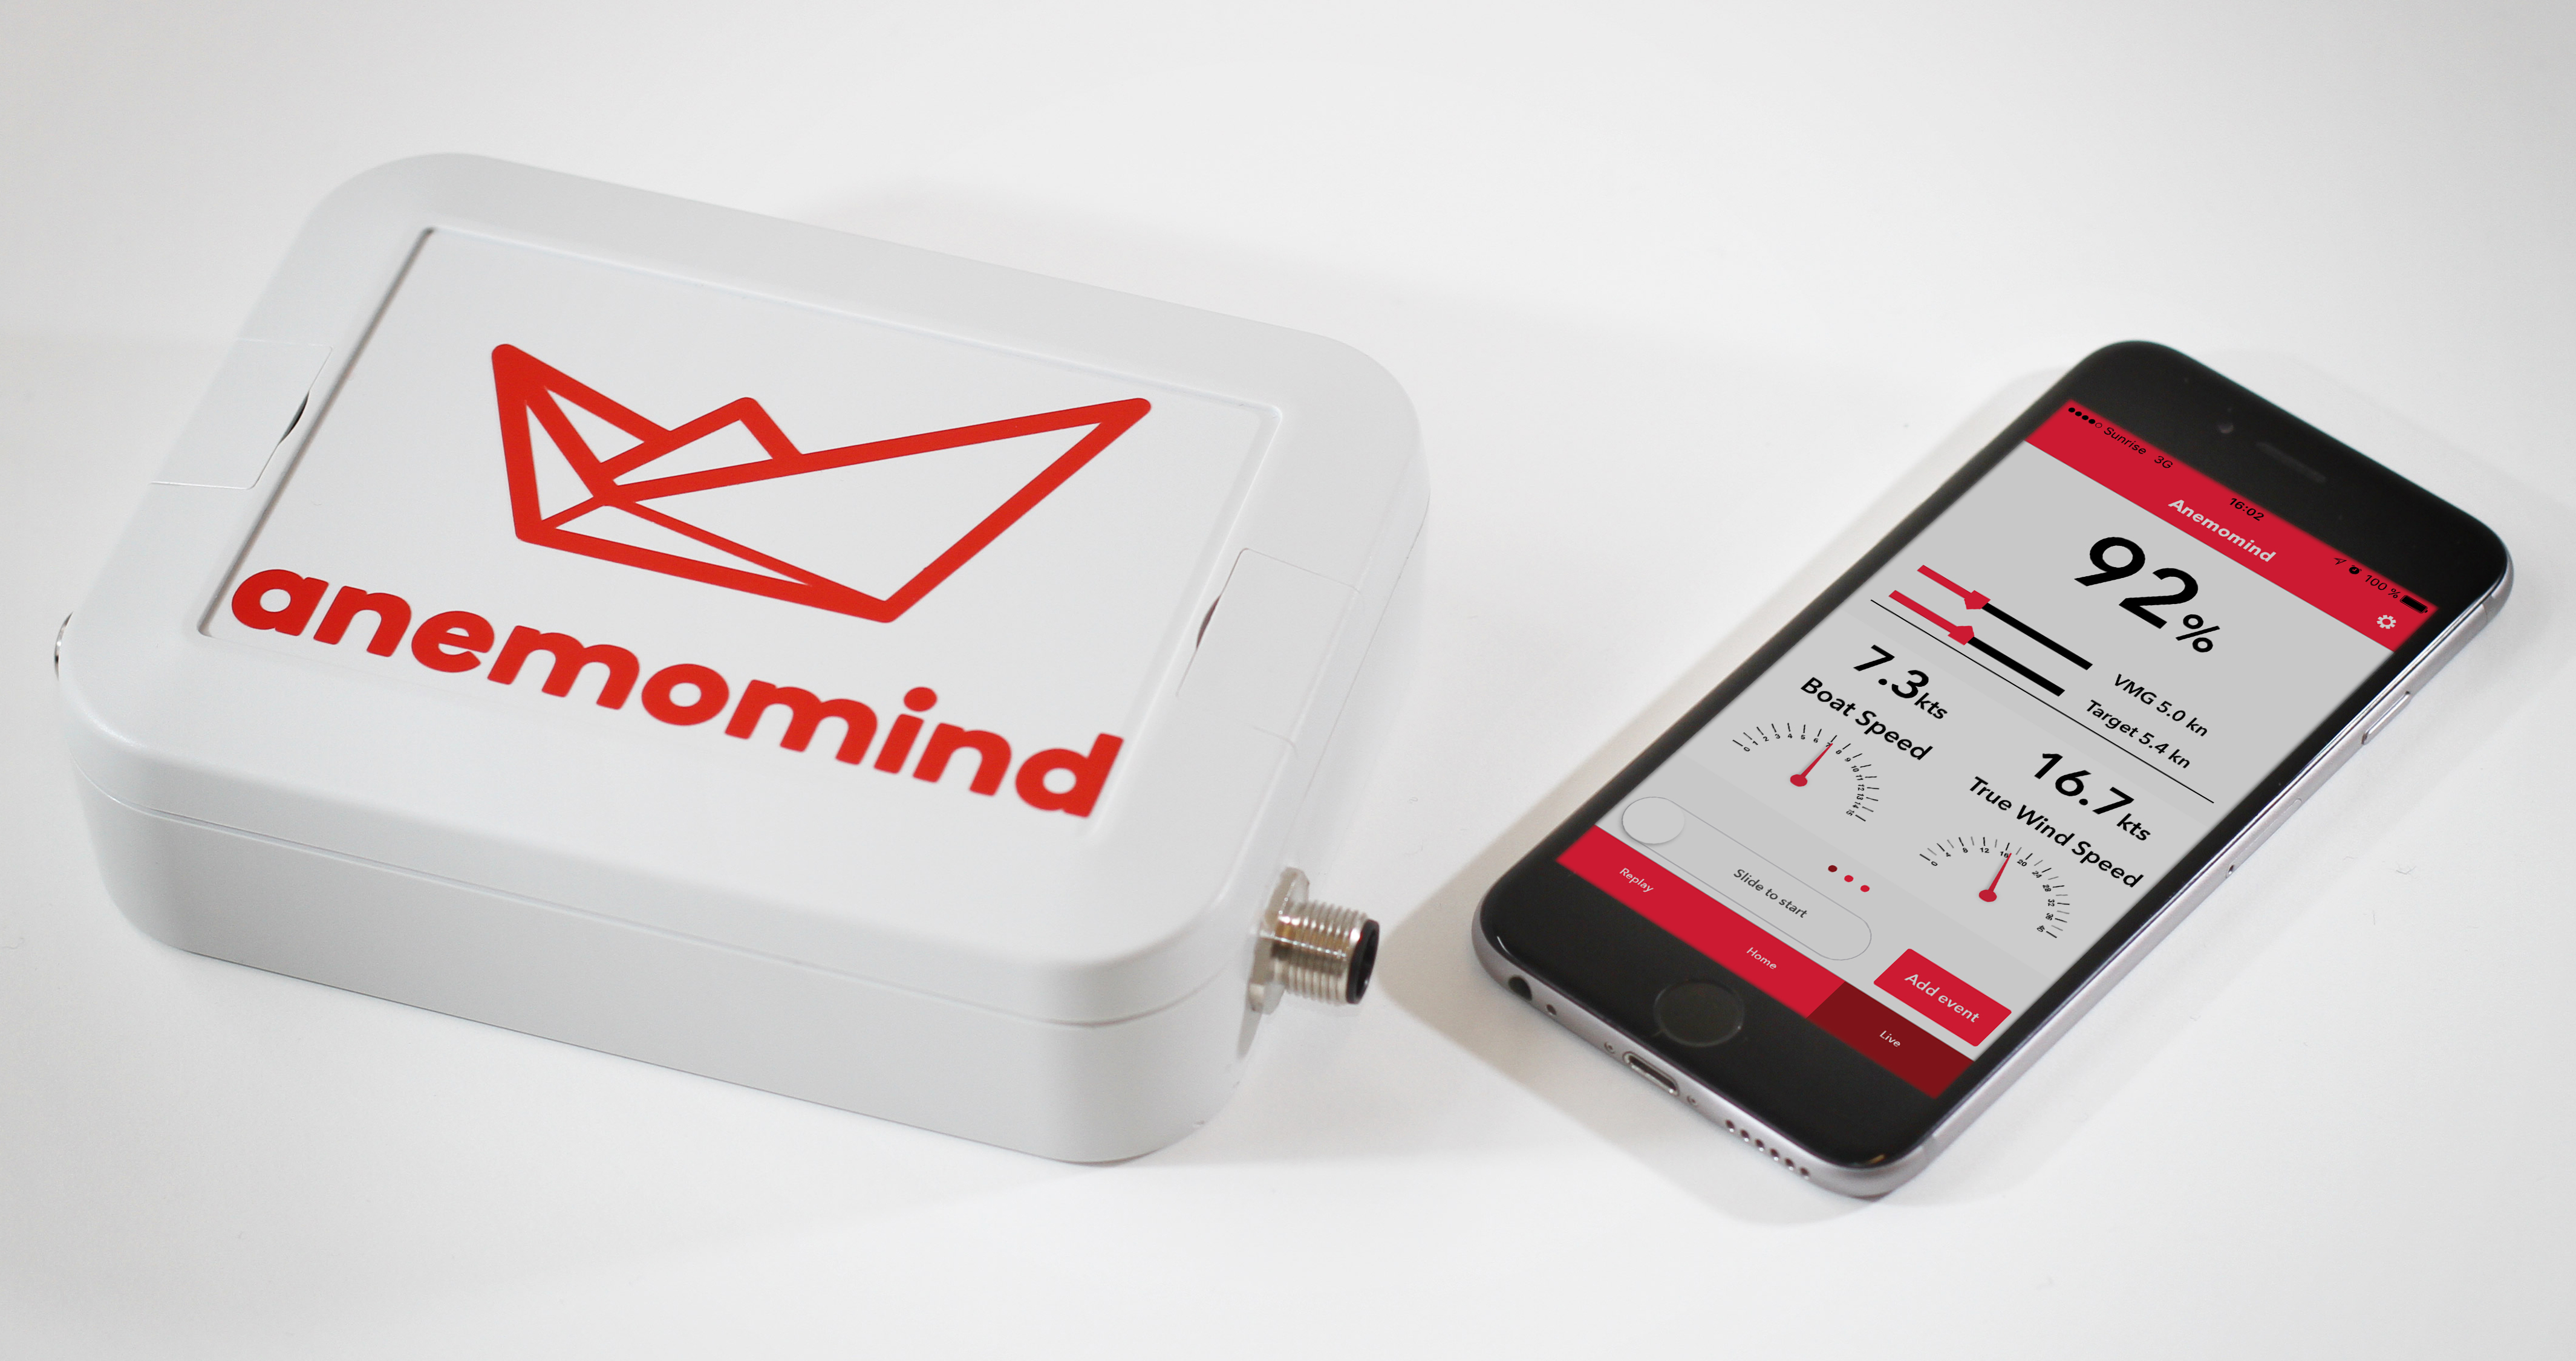
\includegraphics[width=\the\colwidth]{../images/anemobox10.jpg}
  The Anemobox is the heart of the Anemomind system. It is a small onboard computer that captures data from sensors via NMEA. Those data are recorded to log files for deep analysis but also available in real-time via WiFi from your tablet or phone.
}

\anemoparagraph{\the\haligniii}{\the\valigniv}{
  \subheader{The services}
  The cloud-based services and connectivity to iOS devices are what sets Anemomind apart from most existing systems, enabling real-time feedback, as well as a rich analysis and social experience. The services come in three versions: \emph{Social sailors}, \emph{Amateur racers} and \emph{Professional racers}. You can either subscribe to these services per year or lifetime.
  
  \bigskip

  \begin{tabularx}{\colwidth}{|X|c|c|c|}
    \hline
    & \roth{Social sailors} & \roth{Amateur racers} & \roth{Professional racers} \\ \hline
    Public navigation sharing & \OK & \OK & \OK \\ \hline
    Unlimited navigation data storage & \OK & \OK & \OK \\ \hline
    Performance estimation & & \OK & \OK \\ \hline
    Full instrument display & & \OK & \OK \\ \hline
    VMG table & & \OK & \OK \\ \hline
    Private sharing with team & & & \OK \\ \hline
    Raw data export (CSV) & & & \OK \\ \hline
  \end{tabularx}
}


%% https://www.senero-marine.ch/wp-content/uploads/2017/01/BandG_Preisliste_2017.pdf
\anemoparagraph{\the\haligni}{\the\valigniv}{
  \subheader{Compose your package}
}


\node[anchor=south west,style={inner sep=0,outer sep=0}] at (0cm,0cm) {
  \begin{minipage}[l]{\the\dimexpr(1.05\colwidth)}
    \includegraphics[width=\textwidth]{../priceflowchart.pdf}
  \end{minipage}
};

\node[anchor=south east,style={inner sep=0,outer sep=0}] at (\the\contentswidth,0cm) {
  \begin{minipage}[l]{3.5cm}
    
\includegraphics[width=\textwidth]{../images/logosmall.pdf}
  \end{minipage}
};

\anemoparagraph{\the\haligniii}{\the\valignii}{
  \subheader{Anemobox Specs}
  %\rowcolors{2}{gray!25}{white}
  {
    \scriptsize
    \spectable{Embedded sensors}{
      GPS networks & multi-GNSS (GPS/QZSS, GLONASS and BeiDou) \\
      GPS accuracy & 2.5 m CEP \\
      GPS Frequency & 1-10 Hz \\
      External GPS support & NMEA 0183 and 2000 \\
      Inertial Measurement Unit &	9 axis, 1 kHz \\
      Compass & 3 axis magnetometer, compensated with 3 gyroscopes \\
    }
    \spectable{Processing Characteristics}{
      Processing & dual-core, dual-threaded Intel® Atom CPU at 500 MHz \\
      RAM & 1 GB \\
      Logging storage & 8 GB \\
      System storage & 4 GB \\
    }
    \spectable{Connections}{
      Wireless & Wifi, Bluetooth 4.0 \\
      8-poles IP67 connector & Power, NMEA input + output \\
      NMEA 2000 connector & Power, data input + output \\
    }
    \spectable{Physical Characteristics}{
      Size & 11 $\times$ 15 $\times$ 4 cm \\
      Weight & 227 g \\
    }
    \spectable{Electrical Characteristics}{
      Supply voltage & 9--24 V DC \\
      Power consumption & 1.5 W \\
      Current at 12 V & 0.12 A \\
    }
  }
  \rowcolors{2}{white}{white}
}
\end{tikzpicture}
\end{document} 

